%!TEX root = ../../main.tex
\section{Specifikation og Analyse}
I vores overvejelser omkring systemet har vi lagt vægt på at det skulle kunne virke over lange afstande og at brugeren sjældent skal have behov for at skulle tilgå hardware ved kar og sensor ø, det skulle således kun ske ved når der skal tilføjes nye sensorer eller nye sensorøer. \\
Desuden skulle bruger grænsefladen være nemt at tilgå, det gik også op for os at det var en god ide at have system inddelt således at bruger grænsefladen stod for sig selv da systemet så kan udvides med flere kar, samme argumentation gælder for sensorøen da et kar kan stå for at vande mange planter og det giver god mening at kunne opsamle data flere steder fra og det giver mulighed for bedre at styre vand mængden til forskellig områder af planteområdet.

\begin{figure}[H]
	\centering
	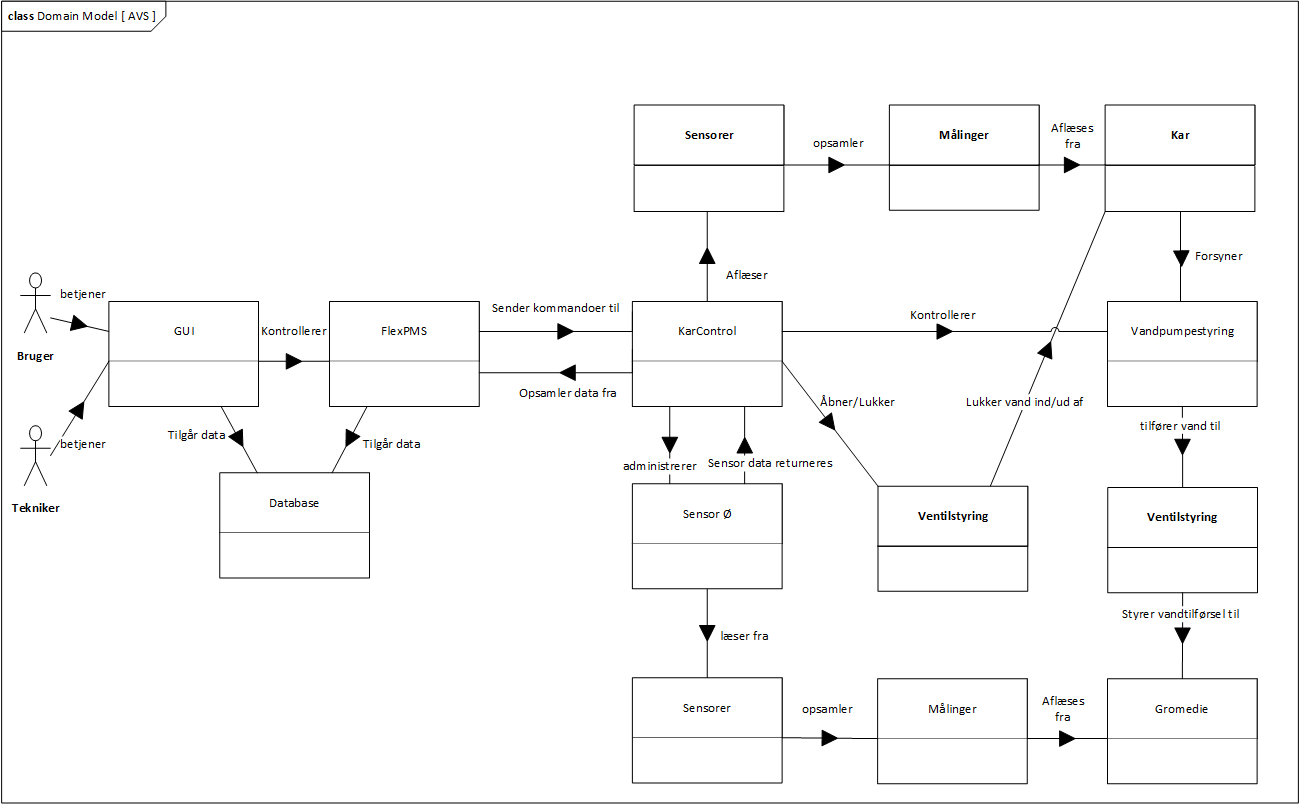
\includegraphics[width=1\textwidth]{Projektbeskrivelse/SpecifikationOgAnalyse/System_Domain_Model.png}
	\caption{Domæne model for AVS}
	\label{fig:DomaeneSys}
\end{figure} 

På modelen herover\ref{fig:DomaeneSys} ses et udlæg af systemet her er det lidt svært at se at systemet er meget opdelt, men modellen illustrer data vejen i systemet hvordan systemet samler data op som det skal bruge til at logging og automatisk vanding.
\\
På baggrund af disse tanker har vi valgt at bruge en bus med differentielt signal til at opnå afstandene i systemet, desuden har vi valgt selv at designe vores sensorer.